	\begin{enumerate}
		\item How many different ways are there to place the dominoes in a $2\times n$ hallway?
		
		$n=1$
		\begin{tikzpicture}[scale=2]
			\draw (0 ,0 ) -- (0 , 2  ) -- (1 , 2  ) -- (1 ,0 )--cycle;
		\end{tikzpicture} \hfill
		$n=2$
		\begin{tikzpicture}[scale=2]
			\draw (0 ,0 ) -- (0 , 2  ) -- (2 , 2  ) -- (2 ,0 )--cycle;
		\end{tikzpicture}
		\hfill
		$n=3$
		\begin{tikzpicture}[scale=2]
			\draw (0 ,0 ) -- (0 , 2  ) -- (3 , 2  ) -- (3 ,0 )--cycle;
		\end{tikzpicture}

		$n=4$
		\begin{tikzpicture}[scale=2]
			\draw (0 ,0 ) -- (0 , 2  ) -- (4 , 2  ) -- (4 ,0 )--cycle;
		\end{tikzpicture}

		$n=5$
		\begin{tikzpicture}[scale=2]
			\draw (0 ,0 ) -- (0 , 2  ) -- (5 , 2  ) -- (5 ,0 )--cycle;
		\end{tikzpicture}
		
			$n=6$
		\begin{tikzpicture}[scale=2]
			\draw (0 ,0 ) -- (0 , 2  ) -- (6 , 2  ) -- (6 ,0 )--cycle;
		\end{tikzpicture}
		\item What would be a formula for a general $n$?  Explain why the pattern and formula work.
		
\clearpage
		\item There are three ways to dissect a $3\times 2$ rectangle into
dominos. How many ways are there to dissect a $3\times 4$ rectangle into dominos?

\begin{tikzpicture}[scale=2]
			\draw (0 ,0 ) -- (0 , 3  ) -- (4 , 3  ) -- (4 ,0 )--cycle;
\end{tikzpicture}
		
	\item It is not possible to dissect a $3\times1$ rectangle into dominos. Likewise it is not possible to
dissect $3\times3 3\times5, 3\times7$,… rectangles into dominos. Suppose we remove a single $1\times1$
square from the lower left corner of these rectangles (we’ll call these shapes the $3\times1-
1, 3\times3-1, 3\times5-1$,…). These shapes can be dissected into dominos. Below we show, for
example, how to dissect the $3\times1-1$ shape, $3\times3-1$ shape, and $3\times5-1$ shape into dominos.
How many ways are there to dissect a $3\times3-1$ rectangle into dominos? A $3\times5-1$
rectangle into dominos?

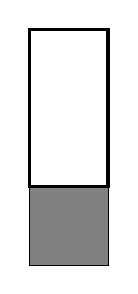
\begin{tikzpicture}[scale=1]
			\draw (0 ,0 ) -- (1 , 0) -- (1 , 3) -- (0 , 3)--cycle;
			\draw[fill=gray] (0 ,0 ) -- (0 , 1) -- (1 , 1) -- (1 ,0 )--cycle;
			\draw[very thick] (0, 1) -- (1 , 1) -- (1 , 3) -- (0 , 3)--cycle;
\end{tikzpicture} \hfill
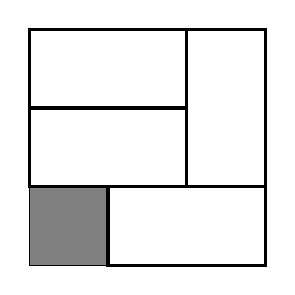
\begin{tikzpicture}[scale=1]
			\draw (0 ,0 ) -- (3 , 0) -- (3 , 3) -- (0 , 3)--cycle;
			\draw[fill=gray] (0 ,0 ) -- (0 , 1) -- (1 , 1) -- (1 ,0 )--cycle;
			\draw[very thick] (1, 0) -- (3 , 0) -- (3 , 1) -- (1 , 1)--cycle;
			\draw[very thick] (0, 1) -- (2 , 1) -- (2 , 2) -- (0 , 2)--cycle;
			\draw[very thick] (0, 2) -- (2 , 2) -- (2 , 3) -- (0 , 3)--cycle;
			\draw[very thick] (2, 1) -- (3 , 1) -- (3 , 3) -- (2 , 3)--cycle;
\end{tikzpicture}\hfill
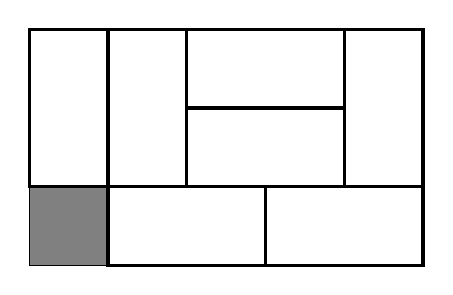
\begin{tikzpicture}[scale=1]
			\draw (0 ,0 ) -- (5 , 0) -- (5 , 3) -- (0 , 3)--cycle;
			\draw[fill=gray] (0 ,0 ) -- (0 , 1) -- (1 , 1) -- (1 ,0 )--cycle;
			\draw[very thick] (1, 0) -- (3 , 0) -- (3 , 1) -- (1 , 1)--cycle;
			\draw[very thick] (3, 0) -- (5 , 0) -- (5 , 1) -- (3 , 1)--cycle;
			\draw[very thick] (0, 1) -- (1 , 1) -- (1 , 3) -- (0 , 3)--cycle;
			\draw[very thick] (1, 1) -- (2 , 1) -- (2 , 3) -- (1 , 3)--cycle;
			\draw[very thick] (2, 1) -- (4 , 1) -- (4 , 2) -- (2 , 2)--cycle;
			\draw[very thick] (2, 2) -- (4 , 2) -- (4 , 3) -- (2 , 3)--cycle;
			\draw[very thick] (4, 1) -- (4 , 3) -- (5 , 3) -- (5 , 1)--cycle;
\end{tikzpicture}

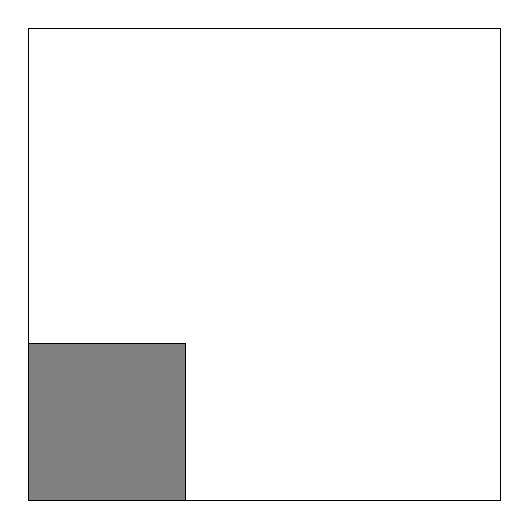
\begin{tikzpicture}[scale=2]
			\draw (0 ,0 ) -- (3 , 0) -- (3 , 3) -- (0 , 3)--cycle;
			\draw[fill=gray] (0 ,0 ) -- (0 , 1) -- (1 , 1) -- (1 ,0 )--cycle;
\end{tikzpicture}
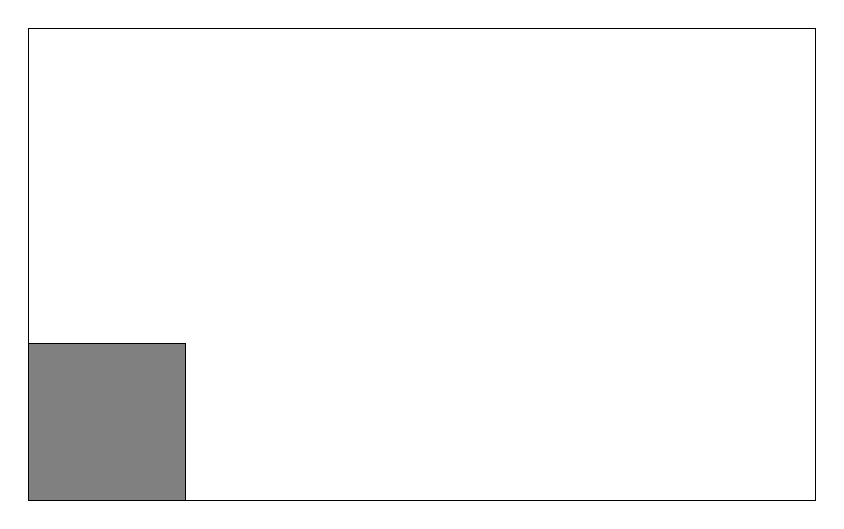
\begin{tikzpicture}[scale=2]
				\draw (0 ,0 ) -- (5 , 0) -- (5 , 3) -- (0 , 3)--cycle;
			\draw[fill=gray] (0 ,0 ) -- (0 , 1) -- (1 , 1) -- (1 ,0 )--cycle;
\end{tikzpicture}
	\end{enumerate}
	\clearpage
	


\begin{tikzpicture}[scale=1.9]
\foreach \y in {0,2,...,10}
\foreach \x in {0,1,...,7}{
			\draw (\x ,\y ) -- (\x , 2+\y  -.1) node[pos=.5] (1) {} -- (\x +1  -.1, 2+\y   -.1) -- (\x +1  -.1, \y )  node[pos=.5] (2) {}--cycle;
			\draw[dashed] (1)--(2);}
		
	\end{tikzpicture}
	\clearpage
